\section{Módulo do Motor}\label{sec:modulo_motor}

Os módulos de motor (Figura~\ref{fig:modulo_motor}) fazem o controle dos quatro motores responsáveis pelo movimento do robô e do motor responsável pela atuação do driblador. Cada módulo consiste em uma ponte H capaz de controlar a velocidade de um motor de corrente contínua em duas direções. 

\begin{figure}
	\centering
	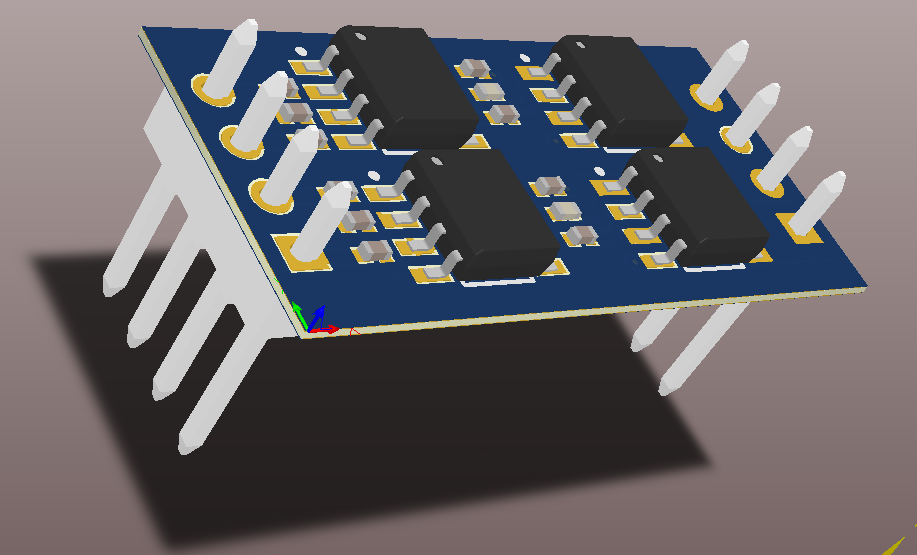
\includegraphics[scale=1]{modulo_motor}
	\caption{Módulo de Motor}
	\label{fig:modulo_motor}
\end{figure}

\begin{figure}
	\centering
	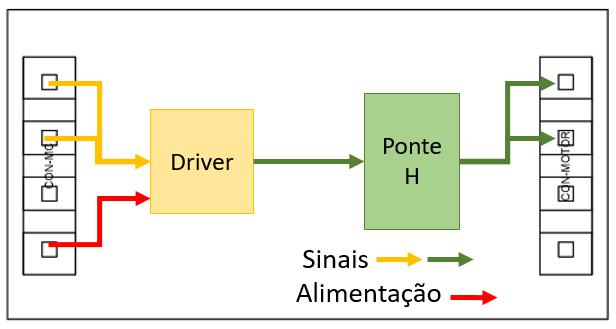
\includegraphics[scale=1]{blocos_motor}
	\caption{Diagrama de blocos do módulo de motor}
	\label{fig:blocos_motor}
\end{figure}

Esta placa é controlada pelo módulo de controle através da classe motor que utiliza a classe encoder para determinar a velocidade instantânea do motor. Com essa velocidade utiliza-se um algoritmo de controle PID para calcular a resposta que deve ser transmitida à placa, e envia-se essa resposta utilizando as classes degrau unitário e PWM.
O circuito de ponte H permite que o microcontrolador controle o sentido de rotação dos motores e a potência transmitida a eles, através do chaveamento dos transistores internos da ponte e amplificando o sinal enviado pelo microcontrolador.
O desenho dessa placa foi reformulado esse ano, as trilhas foram trocadas por planos nos caminhos de potência e foram adicionados um par de capacitores de desacoplamento na entrada dos drivers dos transistores.


% vim: tw=80 et ts=2 sw=2 sts=2 ft=tex spelllang=pt_br,en
